\documentclass[11pt]{jarticle}

\usepackage[dvipdfmx]{graphicx}

\setlength{\oddsidemargin}{-6.35mm}
\setlength{\textwidth}{171.9mm}

\begin{document}

\title{画像処理実験 第5回}
\author{09430509\\今田将也}
\date{\number\year 年\number\month 月\number\day 日}
\maketitle

\section{極大値を探し出し,その座標を配列に記録する部分を完成}

外側の2重ループで,x方向とy方向の走査をしている.
中身でWに対応する短形領域内での最大値を探す.Wはコマンドライン引数から与えることができる.
このとき,Wの値が小さすぎると,点が出てこずにセグメンテーションフォールトが起きてしまう.

そして,最大値が操作している点と同じならそこを特徴点として記録している.以下そのソースコードである.

\begin{verbatim}
    for(y=W+1;y<im2->H-W-1;y++){
        for(x=W+1;x<im2->W-W-1;x++){
          double max=-1;
          for(v=-W;v<=W;v++){
            for(u=-W;u<=W;u++){
              // (x,y) を中心とする 15x15 の矩形領域内で DElem(im2,x+u,y+v) の最大値を探す.
              if(DElem(im2, x+u, y+v) > max){
                max = DElem(im2,x+u,y+v);
              } 
            }
          }
          // 最大値が DElem(im2,x,y) と等しいなら,(x,y) を特徴点として記録する. 
          if(max == DElem(im2,x,y)){
            a = n++; 
            w[a][0] = x;
            w[a][1] = y;
            w[a][2] = max;
          }
        }
      }
\end{verbatim}

\section{得られた極大点リストから,「特徴点らしさ」の大きいものを N 個選び出す}

ここでは,qsort関数を用いてソートをした.

\begin{verbatim}
    qsort(kk, kw, sizeof(kk[0]),desc);
\end{verbatim}

kkは予め宣言されている配列で,kwはMatrixLocalMaxの返り値として赤い点の個数が与えられている.要素の1つ分はx,y,maxについて3つ分あるのでkk[0]で記載.
descという関数は降順に並び替えるものである.
\begin{verbatim}
    int desc(int left[3], int right[3])
    {
      return right[2]-left[2];
    }
\end{verbatim}

出力された点を一部抜粋すると,maxの値で降順に並んでいる.
\begin{verbatim}
    383 465 790611
    614 440 755117
    354 500 745975
    403 462 714745
    242 528 701629
    295 498 656782
    687 482 626184
\end{verbatim}

\begin{figure}[ht]
  \centering
  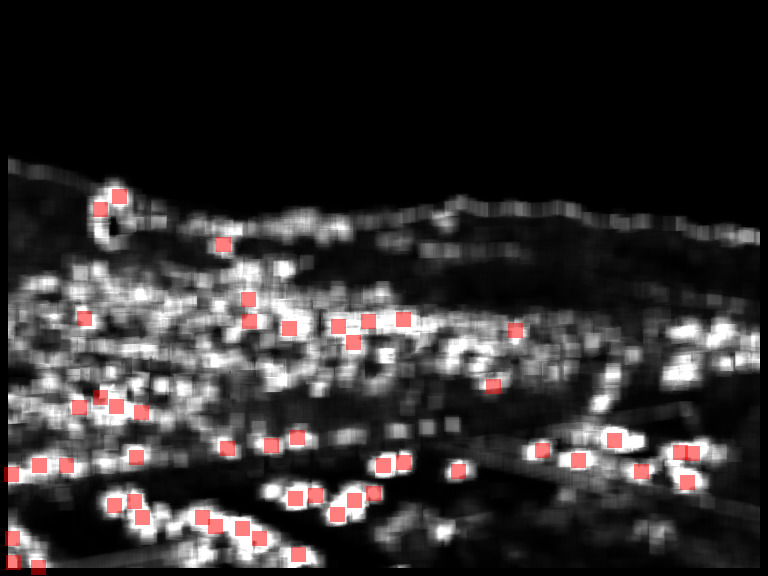
\includegraphics[scale=.3]{50.jpg}
  \caption{50個}
\end{figure}

\begin{figure}[ht]
  \centering
  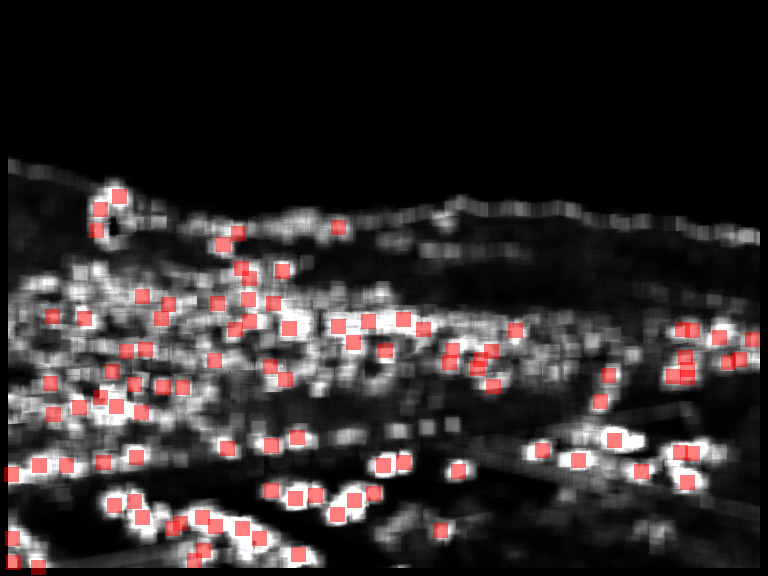
\includegraphics[scale=.3]{100.jpg}
  \caption{100個}
\end{figure}

\section{速度とメモリを効率化}
実装例で確保された領域 int kk[9999][2] の要素数は,検出され得る最大数より遥かに少なく問題が起きる可能性があると資料にあるのはうなずける.
また,画素数と同数の作業領域を確保するのは無駄が多い.
そこで資料を参考に,現在までに発見された点を,MAX 個まで保持できる領域を用意し,MAX+1 個目以降の追加時には,新しい候補か現在の最下位候補のどちらかを破棄することで,候補が MAX 個を越えない様にする.
実装には挿入ソートを用いた.以下そのソースコードである.

\begin{verbatim}
    for(v=-W;v<=W;v++) for(u=-W;u<=W;u++){
        if(DElem(im2, x+u, y+v) > max){
          max = DElem(im2,x+u,y+v);
        }
      }
      if( max == DElem(im2, x, y) ){
        a = n;
        if(n < MAX) { n++; }
        for(;a>0 && w[a-1][2] < DElem(im2, x, y);a--){
          w[a][0]=w[a-1][0]; w[a][1]=w[a-1][1]; w[a][2]=w[a-1][2];
        }
        w[a][0]=x; w[a][1]=y; w[a][2]=max;
      }
\end{verbatim}

\section{感想}

コマンドラインから短形領域を変更することで,特徴点の位置が変わったり,出す特徴点の個数に限界をもたせることでメモリの効率化ができることは
理解できた.前回はなんとかできた分解,あまり理解をできていなかったため今回は実装ができず速度の効率化については調べることができなかった.
また,並列化やGPUでの実装には全く手をつけていないので余裕があれば行いたいが,かなり毎回のレポートがギリギリなのでできないと思う.
\end{document}
